\documentclass[a4paper, 12pt]{report}
\usepackage[english]{babel}
\usepackage{blindtext}
\usepackage[a4paper, inner=2.5cm, outer=3cm, top=3cm, bottom=3cm]{geometry}
\usepackage{fancyhdr}
\usepackage{mathtools}
\usepackage{amssymb}
\usepackage[toc,page]{appendix}
\usepackage{hyperref}

\fancyhf{}
\fancyhead[LE]{\leftmark}
\fancyhead[RO]{\nouppercase{\rightmark}}
\fancyfoot[C]{\thepage}
\pagestyle{fancy}

\usepackage{graphicx}
\graphicspath{ {report/images/} }

\begin{document}

\begin{titlepage}
    \begin{center}
        \Huge
        \textit{Linear Programming\\to\\Solve Vehicle Routing Problem}

        \vspace{1.5cm}

        
\includegraphics[width=0.4\textwidth]{ucl-logo.jpg}
        
        \vspace{1.5cm}
        
        \Large
        Submitted by:\\
        Muhammad Rafdi\\

        \vspace{0.8cm}

        Department of Computer Science\\
        University College London\\
        London\\
        29 April 2016

        \vspace{0.8cm}
        Supervised by:\\
        Dr Daniel Hulme       
        
        \vfill
                
        
        \normalsize   
        This report is submitted as part requirement for the BSc Degree in Computer Science at UCL. It is substantially
         the result of my own work except where explicitly indicated in the text. The report may be freely copied and
          distributed provided the source is explicitly acknowledged.

        
    \end{center}
\end{titlepage}

\newgeometry{inner=1.5cm, outer=3cm, top=2cm, bottom=3cm, bindingoffset=1cm}

\begin{abstract}
\centering
   This project examine the state of the art of linear programming and how to formulate combinatorial optimisation
   problems in terms of linear programs. We examine a specific problem : The vehicle routing problem and solve a
   few instances of it based on a given data set using different solvers. The results are then studied thoroughly.
\end{abstract}

\renewcommand{\abstractname}{Acknowledgements}
\begin{abstract}
\centering
I would like to thank Dr Daniel Hulme for his support and encouragement. Guan Yang Song and etc...
\end{abstract}

\tableofcontents
\
% chapter 1
\chapter{Introduction}
Linear Programming is a mathematical method to find an optimal value of a function in a linear system under a set of
constraints. This method has been around since the 19th century, but it was not fully developed until the World War 2,
where it was used for resources planning. Since its conception, this method has been widely used to solve problems
in Applied Mathematics and Operations Research (OR). Along with the advancement of computing, companies can now increase their
decision making capabilities with efficient technique of linear programming and significant computational power.

Linear programming is used to model to many combinatorial problems, such as vehicle routing.
The vehicle routing problem is a common problem that is commonly observed in logistics.
It is a special instance of the famous traveling salesperson problem in which the tour of
all 'cities' in the given graph into several parts, subject the availability of resources.

In this project, we will conduct an Operations Research study by using linear programming to find the optimal routes of an instance of a vehicle routing
problem. We will use three linear programming tools to arrive at a solution and compare and contrast the results of each one of them.

\section{Project Motivation}
Linear programming has allowed organisations to optimise many aspects its operations. In many occasions, the problem involves
finding the optimal combination of input that yields the greatest output. Amongst the many problems,
vehicle routing is one of them. Many studies have been carried out on this problem due to its role in minimising operational
costs of companies, especially in their logistics department. Logistic plays a significant role in many businesses and it is one of the major
driving force of the economy. In the UK alone, Logistics and Posts Sector is worth approximately
\pounds55bn to the economy and comprises 5 percent of the GDP\footnote{According to a logistics report by PWC }.
In the US, the cost attributed to logistics rose up to US\$1.45 trillion in 2014, an increase of 3.1 percent from the previous year.
These figures are likely to increase given the increasingly globalised economy. Thus, minimising operational costs will not only make companies
more competitive, but it will also increase their profits. In this project, we want to simulate a scenario where we can optimise
a problem to minimise cost in a fictional delivery company DFFS. We will demonstrate how optimisation can help them solve a vehicle
routing they face.

Aside from financial benefits, the vehicle routing problem is an interesting problem to the mathematically and computationally apt individuals.
There are wide variety of algorithms that can be used to approximate the optimal solution.

A study on the comparison of solvers has been done before in \[inser bib here\]. However, it does not include other open souce LP tools
such as or-tools and Optaplanner, both of which contains their own unique engine to solve LP problems. It will be useful to see the comparison
of different tools as it will help OR analysts to decide which tool is the best for them given their current needs. We have chosen the 3 tools mentioned
because they are relatively popular tools used in the industry there that is relatively well documented and
has an easy to use APIs in various programming languages including Python, the language that we use in this project. Most importantly, they have not
been compared alongside one another.

\section{Goals and Scope of Project}
We have identified a few goals to benchmark this project and a scope to limit the discussions that may have been related to this project. The goals are as
follows:
\begin{enumerate}
\item To thoroughly understand linear programming method to solve optimisation problems.
\item To build a mathematical model of the vehicle routing problem based on the given dataset.
\item Obtain the optimised results (the minimum distance and the paths) using the chosen tools.
\item Compare and contrast the results and the usage of those tools.
\end{enumerate}

Creating novel algorithms for optimisation problems is hard and requires years of experience in Algorithms.
Implementing linear programming solver is also difficult and it requires very high level of software engineering expertise, in addition to
the algorithmic knowledge mentioned. For these reasons, we will not be attempting to create new algorithms or implement linear programming solvers to solve
the vehicle routing problem. Instead we will model the VRP instance using softwares and algorithms that are already available.
In addition, other methods that can be used to solve this problem such as \textit{genetic programming} and \textit{dynamic programming} will
not be covered in this project.

\section{Methodology}
Peforming the calculations for linear programming is not as hard as it used to be given the availability of computing power that we have today.
In this project we will be using three applications: Gurobi, OR Tools by Google and Optaplanner to retrieve the optimal solution. Each of them
contains their own implementation of \textbf{linear programming solver}, a program that can solve linear programming problems. We model them
in a form that can be solved by these solvers and used the solvers to obtain the solution.

This project will be carried out in seven steps, as per the steps taken in a typical OR study:

\begin{enumerate}
\item Define the problem in a given system and formulate it into a linear program. A linear program is a problem that can be solved
using linear programming. In this step, the objective and the constraints of the system is studied thoroughly to ensure
that the program models the given problem correctly.
\item Collect the data that represents the problem at hand and estimated the parameters that are required to produce
the optimal result.
\item Create the mathematical models of the given problem. We will use standard linear programming notation to build these models. This is
also the step in which we implement the linear program using the chosen softwares.
\item Verify that the model is correct. We achieve this by running the implemented linear program through a benchmark dataset with known solution.
\item Select suitable alternative. We may not always get the desired answer, due various reasons such as limited timescale and computing resources.
In this case, we want to select an alternative objectives that will be useful to the parties involved.
\item Run the given problem in the models that we have build and record their result and performance. We may need to go back to step 1 if the results obtained
are not satisfactory.
\item Provide recommendations to the parties involved based on the results obtained.
\end{enumerate}

For comparing the performance of different linear programming tools, we use a 60 node CVRP model. Time limit of 5 minutes is imposed
when running the model on all tools. The optimal distances obtained using each tools will be recorded and compared. In addition, the usage
of the tools will also be discussed.

We use a lot of terminologies interchangeably here such as blah blah blah. This serves as a heads up to the reader... more explanation needed here..

\section{Outline}
In chapter 2, we will elaborate the underlying theory behind linear programming and its state of the art.
The vehicle routing problem will be discussed in detail in chapter 3. The implentation of linear programming to solve the vehicle routing problem will be
discussed in chapter 4, followed by the results in chapter 5. Finally, I will conclude the results and identify potential future works
of this project in chapter 6.

% chapter 2
\chapter{Theory}
Before we proceed the actual content of the study, it is useful to introduce some theories that will help the reader
to understand the concepts mentioned in the rest of this project. In this section, we will discuss the basics of
linear programming and basic algorithms used for solving them. We will
also discuss briefly how constraints programming is implemented in linear programming solver software.

\section{Linear Programming}
Linear programming is a mathematical method that is commonly used to retrieve an optimal solution from model
that has been converted into a linear system. This model is achieved when all of the mathematical relationship in the model
uses linear functions exclusively. The word 'programming' is not to be confused with the term used in computer science,
in which concerns with formulating instructions for computers to execute. A linear programming system (also called linear
program) consists of three entities:
\begin{enumerate}
\item \textbf{Decision variables} - These are the entities that can be controlled by the decision maker.
\item \textbf{Objective function} - This is the function that, given the optimal input, outputs the optimal value.
In most cases, it is to find the minimum or the maximum value.
\item \textbf{Variable constraints} - These are the restrictions that are imposed on the decision variables. There are two types
of constraints: hard and soft. Hard constraints are constraints cannot be violated at all cost, whereas soft constraints may be
violated, but should be observed wherever possible.
\end{enumerate}
To further undestand how this works, let's walk through a simple example: Bob is competing in
an eating contest where the objective is to accumulate as much points as possible by eating a combination of hotdogs and burgers.
For each burger and hotdog that Bob ate, he will get 5 and 4 points respectively. It takes him 3 minutes to finish a burger and
2 minutes to finish a hotdog and the contest lasts one hour. Bob can consume 25 food items before his appetite reaches its limit.

Based on the scenario above, we can model this problem in the form of a linear program by following these steps:
\begin{itemize}
\item \textbf{Step 1}: Identify the decision variables. Let \(x\) be the number of hotdogs and \(y\) be the number
of burgers eaten by Bob.
\item \textbf{Step 2}: Determine the objective function. In this scenario, we want to determine the highest possible
points that Bob can achieve in the competition. This can be represented by the equation \(z = 4x + 5y\), where
z is the value of the points accumulated in the competition and the coefficients of the variables represent the points achieved by eating respective
food items.
\item \textbf{Step 3}: Determine the constraints. There are 3 constraints in these problem. Firstly, The amount of
food eaten by bob has to be under 60 minutes. This can be represented by the equation \(2x + 3y \leq 60\). Secondly,
Bob's appetite has a limit of 25 food items, which can be modelled with the equation \(x + y \leq 25\). Lastly,
the number of respective food eaten has to be greater than or equal to 0.
\end{itemize}
Putting it together, we have the following linear program:
\[
  \begin{array}{r@{}r@{}l}
    \text{Maximise z =} \quad &{}4x + 5y \\[\jot]
    \text{Subject to}\qquad &{} 2x +   3y &{} \leq 60 \\
    \qquad &{} x +   \phantom{2}y &{} \leq 25 \\
    \qquad &{} x ,   \phantom{2}y &{} \geq 0 \\
  \end{array}
\]
There are two types of solution that can be produced. A feasible solution is a set of variables that satisfies the constraints
of a linear program. An example of a feasible solution for the above solution would be \(x = 25\) and \(y=0\), which yields 100 points.
Optimal solution is the best feasible solution, such as when \(x = 15\) and \(y = 10\), which gives 110 points. In all cases, we want to
find the \textit{optimal} solution. Also, There are 3 types of outcomes in a linear program:

\begin{itemize}
\item \textbf{Outcome 1} : The feasible region is unbounded, thus the objective function is infinity.
\item \textbf{Outcome 2} : The feasible region is empty, this is usually because the constraints on the variables contradict each other.
\item \textbf{Outcome 3} : There is a feasible region that is also bounded. In this case, an optimal solution exists!
\end{itemize}

\begin{figure}[!ht]
  \centering
    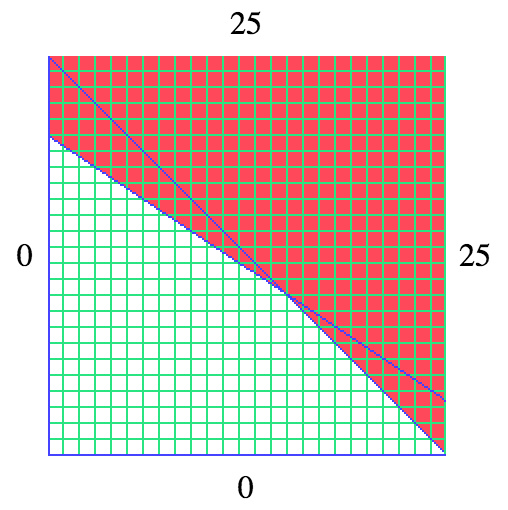
\includegraphics[width=0.5\textwidth]{example-graph.png}
    \caption{Graph representation of a linear program example. The feasible region is shown in white. The optimal solution
  is located at the point (15,10).}
\end{figure}
In order to produce an optimal solution, we can use the simplex algorithm. To understand simplex algorithm, it is best to look at
a graphical representation of the linear program. The simplex algorithm starts off by selecting a point in a graph.
Then it moves to a different point of the graph. On each move, it will make sure that the point yield higher
objective value, by using the values of its axes. If no higher objective value is found, then that point would be the
optimal solution. This method also works in higher dimensional spaces. This explanation is just a simplication of the full
simplex algorithm. The reader may refer to the references section resources that explains the algorithm in detail.

\begin{figure}[!ht]
  \centering
    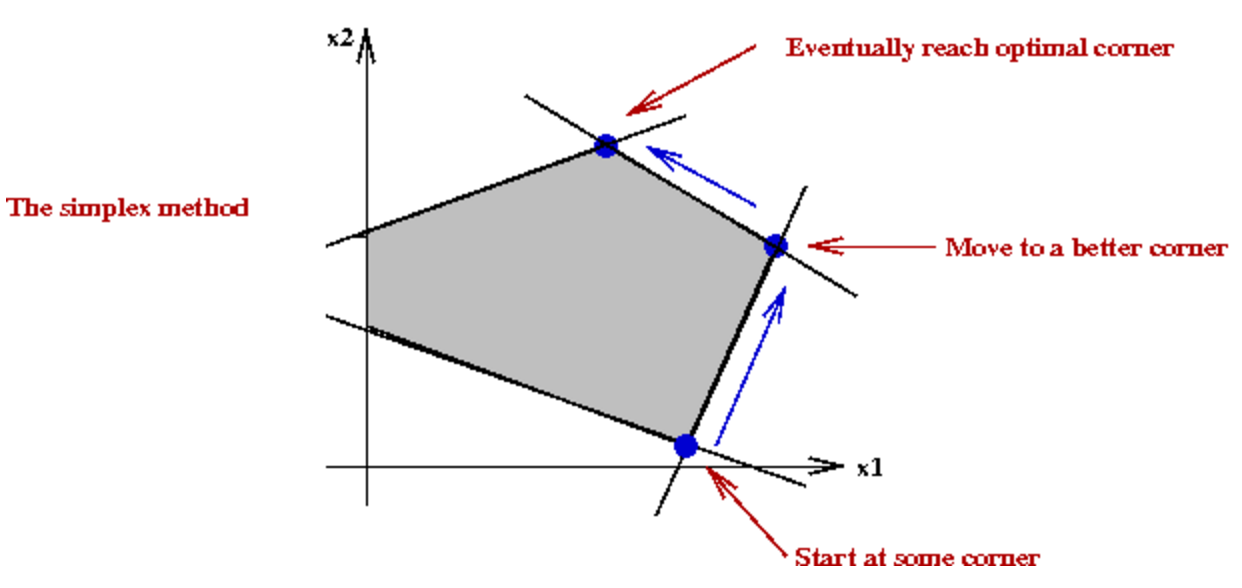
\includegraphics[width=1\textwidth]{simplex.png}
    \caption{Simplex method on a linear program}
\end{figure}

The number of variables in the linear program correspond to the number of dimensions in its graphical representation. For example,
a linear program with 3 variables could be represented by the polyhedra below:

\begin{figure}[!ht]
  \centering
    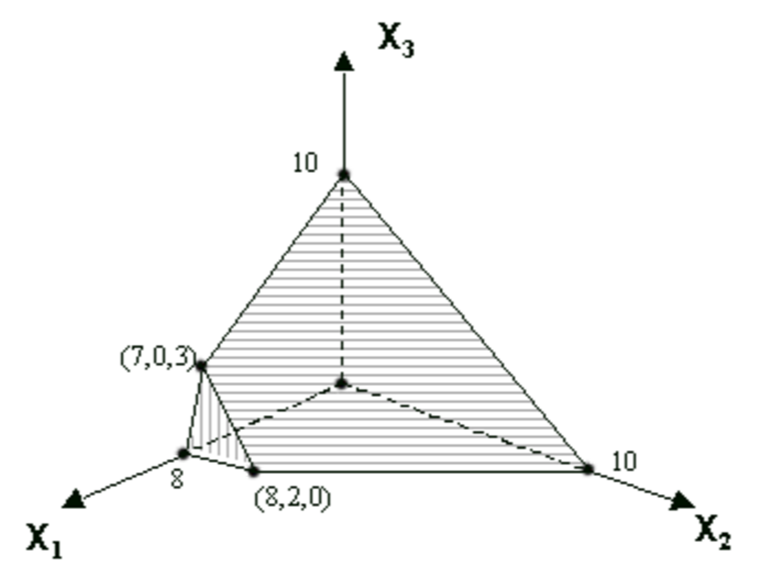
\includegraphics[width=0.5\textwidth]{polyhedra2.png}
    \caption{a polyhedra}
    \vspace{1cm}
    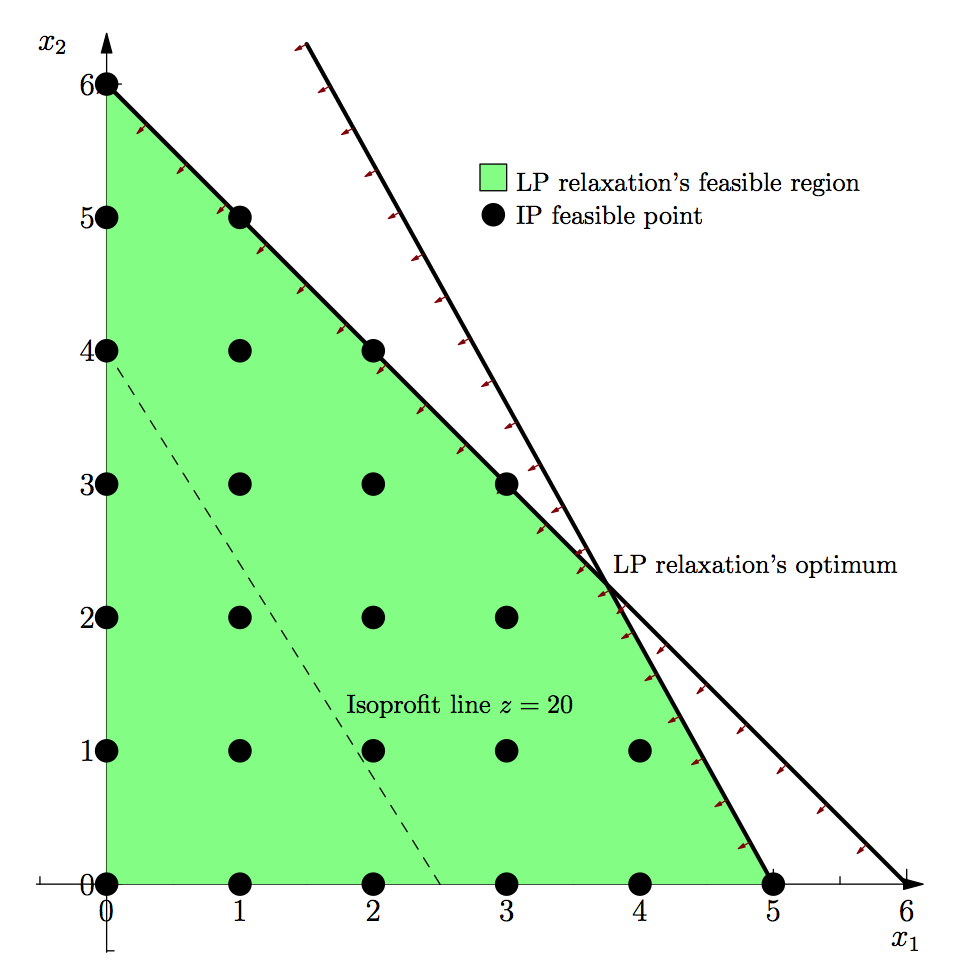
\includegraphics[width=0.5\textwidth]{ipfeasible.png}
    \caption{A graphical representation of a hypothetical linear program. The region bounded by the black line
  line represent the feasible region of the linear program. The region bounded by the blue line represent
   the feasible region of the same linear program, with the addition of itegrality constraint imposed into it.}
\end{figure}

\section{Integer Programming}
Integer programming (also known as integer linear programming) is a system where a linear program has an additional
integrality constraint of imposed on to its decision variables. This is useful in situations where real or
fractional valued variables are not realistic, such as the number of people that it takes to complete a task or the
length of the tour in a hamiltonian cycle.
When this constraint is added, finding an optimal solution becomes harder. This is because the solution can only be
in the lattice points of the graph, thereby
reducing the solution space. Linear programming in which only some of the variables have integrality constraints imposed
into it is known as mixed integer programming (MIP).

More sophisticated algorithms have been invented in order to accomodate the added complexity of IP. One of the most commonly
used algorithm that produces the exact solution is the branch and bound algorithm. It is uses divide and
conquer approach to partition the problem into sub-problems
and then solves them recursively. LP methods such as the simplex can be used to solve the sub-problems.
There are 2 parts to the algorithm: branch and bound. The 'branching' part generates a tree
that continues to expand until all valid solutions are found. The bound part compares all solutions and keeps the
most optimal one.

Let's look at an example to see how it works:
\[
  \begin{array}{r@{}r@{}l}
    \text{Maximise} \quad &{}x_{1} + 12x_{2} \\[\jot]
    \text{subject to}\qquad &{}10x_{1} +   7x_{2} &{} \leq 40 \\
    \qquad &{} x_{1} +   \phantom{2}x_{2} &{} \leq 5 \\
    \qquad &{} x_{1} ,   \phantom{2}x_{2} &{} \in \mathbb{Z}_{>0}\\
  \end{array}
\]

These are the steps of the branch of bound algorithm as it solves the IP problem above:
\begin{itemize}
\item The 'branch' part:
    \begin{itemize}
        \item \textbf{Step 1} : We start by solving the given ILP problem using standard LP method such as the simplex algorithm. Then, we pick the
         variables that does not conform to the integrality constraint as the branching variables. At this point, We are at the root of
         the tree that is generated by this algorithm.
        \item \textbf{Step 2} : Create 2 branches for the chosen branching variable and set a new constraints to that variable in those branches
        . For example, in the children of the root node of the figure 2.5,
         we impose the constraint \(x_{1} \leq 1\) on the left side and \(x_{1} \geq 2\) on the right side of the branch.
        \item \textbf{Step 3} : This is the recursive step of the branching algorithm. We pick a branch and then solve it
        using the same method in step 1. At this point, there are 3 possible outcomes:
            \begin{enumerate}
                \item Infeasible solution: the algorithm will not continue branching from this node and picks other unexplored node
                to solve.
                \item Integral solution found : the algorithm will stop here, record the solution and move on to solve other unexplored node.
                \item Fractional/real solution found: Choose a branching algorithm and then go back to step 2 of this part of the algorithm.
                Exit if there are no explored nodes left.
            \end{enumerate}
    \end{itemize}
\item The 'bound' part: The algorithm will compare all solutions found and keep the most optimal one. The optimal value is set negative infinity at first
and it will be immediately replaced as soon as an integral solution is found.
 This will give the exact solution of the problem.
\end{itemize}

\vspace{0.5cm}

\begin{figure}[!ht]
  \centering
    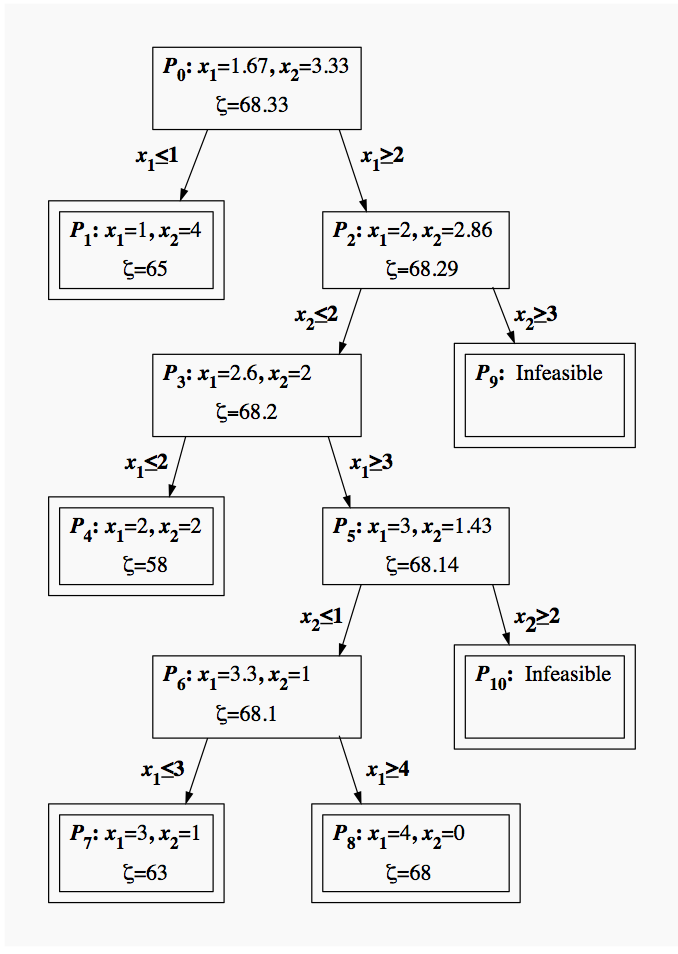
\includegraphics[width=0.6\textwidth]{BNB.png}
    \caption{Enumeration tree that is generated by the branch and bound algorithm for the sample IP problem}
\end{figure}

\section{Constraints Programming}
Unlike the programming that we have observed so far, constraints programming is a programming paradigm that is implemented
in linear programming solvers. Understanding the basics of constraints programming will give insights to how linear programming
solvers work under the hood.

Constraints programming (CP) is a programming paradigm that combines declarative and procedural paradigm. This seems contradictory
at first, because declarative formulation is static whereas a procedural one is dynamic. The idea is boiled down to viewing
a constraint the same way as invoking a procedure. The goal of CP is to find feasible solutions out of large solutions space, making it
more suitable to accomodate LP. Due to this goal, CP focuses on the constraints and variables rather than the objective function.

In this paradigm, a constraint program may be written declaratively but should be viewed as a procedure that operates on a
solution space. Each constraints will be added to a constraint store, which limits the space that must be searched.
Constraint store uses a filtering algorithm that serves as a litmus test for solutions. These solutions will be 'filtered'
by the constraints, which has become part of the constraint store. At the end of the filtering procedure, we obtain a feasible solution.

Given this view, constraint programming formulation tends to look
more like a mathematical programming model than a computer program, since the user writes constraints declaratively
rather than writing procedures to enforce these constraints. For this reason, CP is more suited for solving computer programs that are
LP-based.

% chapter 3
\chapter{Vehicle Routing Problem}
Now that we have covered the basic concepts needed to solve the problem using LP, we shall proceed with
defining the given problem. In this section I will talk about the problem that the company DFFS face and how
we model it with vehicle routing problem model.

\section{Problem Statement}
The company DFFS is a furniture company with more than 30 stores across the UK. At one busy day, the company is scheduled to
make deliveries to 226 customers across the country. Each customers have specific demands for goods. The company has
one depot location, where it stores all of its goods for delivery and 16 delivery vans. The delivery vans only operate on
a time window from 09:00 to 17:00. On each delivery to a customer, it takes an average of 15 minutes for the workers to successfully unload the goods.
The company wants to find the routes that yield the minimum (optimal) distance and such that all customers are visited only once. They are interested
in looking at the optimal distance for both with and without the time windows.
In addition, the company wants to find out if it can use less vans to make all deliveries while keeping the distance roughly the same (or lower if possible) as
the delivery with 16 vehicles.

Modelling this problem to simulate every situations in real life can be difficult and can distract us from focusing on the core problem.
Thus, we may make the following assumptions for convenience:
\begin{enumerate}
\item The service time for all deliveries is set to 15 minutes.
\item All vans are homogeneous and have very large capacity (up to 50 items).
\item All customers have homogeneous demand of 1 item.
\item The delivery vehicles are based in a single depot.
\item The cost of function is set to distance travelled by the vans.
\item Distance from one point to another may be calculated using the haversine formula\footnote{Refer to wikipedia for this}.
\item Traffic conditions are negligible.
\end{enumerate}

\section{Problem Definition}
The problem mentioned above is also known as the vehicle routing problem (VRP), a classic optimisation problem that has been
documented and researched for decades. VRP is a problem where a fleet of vehicles, which are based on a central location (also known
as the depot), are required to visit geographically dispersed customers to fulfil their respective requirements. The main objective is
to find the optimal routes for the fleet of vehicles that yield a minimum cost, which could be in terms of fuel, time or distance.
There are many variants of VRP and they are based on the constraints imposed onto them. A few examples include VRP with multiple depot (MDVRP) and
a VRP where the customers can demand or return services (VRPB).
\begin{figure}[!ht]
  \centering
    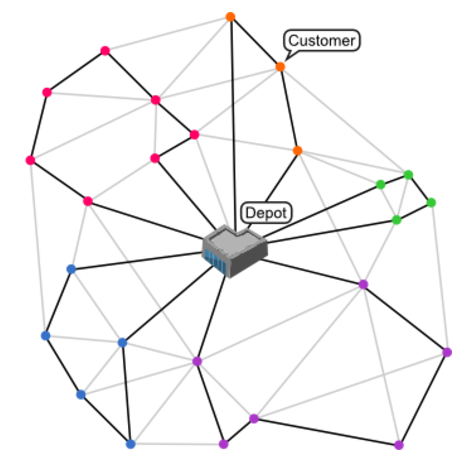
\includegraphics[width=0.6\textwidth]{vrp-sample.png}
    \caption{a visualisation of VRP}
\end{figure}

We can specifically define the problem given in the previous section with two known VRP models: capacitated
vehicle routing problem (CVRP) and capacitated vehicle routing problem
with time windows model (CVRPTW). Both of which have only one depot. The CVRP model has the following input:
\begin{itemize}
\item A complete graph \(G = (V, E)\). which consists of the vertices \(V\) and the edges \(E\).
\item The variable \(n\), which represent the total number of customers and the depot.
\item The variable \(K\), which represent the total number of vehicles available.
\item A vertex set \(V\), numbered from 1 to \(n\) and vertex 1 is the depot.
\item A set of edges for \(V\).
\item The cost function \(c_{ij}\) that outputs the distance travelled from vertex i to j, where \(i,j \in V\).
\item The path function \(x_{ij}\) that outputs 1 if the path i to j is included in the current journey and 0 otherwise.
\item The capacity function \(r(S)\) that outputs the number capacity needed to serve a set of customers \(S\).
\end{itemize}

Given the input above, we can create a single depot capacitated vehicle routing problem below (needs proper alignment):

\vspace{0.5cm}

\begin{equation}
    \begin{array}{ll@{}ll}
        \text{Minimize} & \displaystyle\sum\limits_{i \in V}\sum\limits_{j \in V} c_{ij}&x_{ij} &\\
    \end{array}
\end{equation}
\begin{equation}
    \begin{array}{ll@{}ll}
        \text{Subject to}&\displaystyle\sum\limits_{i \in V}   &x_{ij} = 1,  &\forall j \in V \setminus \{1\}\\
    \end{array}
\end{equation}
\begin{equation}
    \begin{array}{ll@{}ll}
        & \displaystyle\sum\limits_{j \in V}   &x_{ij} = 1,  &\forall i \in V \setminus \{1\}\\
    \end{array}
\end{equation}
\begin{equation}
    \begin{array}{ll@{}ll}
        & \displaystyle\sum\limits_{i \in V}   &x_{1i} = K\\
    \end{array}
\end{equation}
\begin{equation}
    \begin{array}{ll@{}ll}
        & \displaystyle\sum\limits_{i \in V}   &x_{i1} = K\\
    \end{array}
\end{equation}
\begin{equation}
    \begin{array}{ll@{}ll@{}ll}
        & \displaystyle\sum\limits_{i \in S}\sum\limits_{i \in S}  &x_{ij} \leq |S| - r(S), &\forall S \subseteq V/ \{1\} , S \neq \o \\
    \end{array}
\end{equation}
\begin{equation}
    \begin{array}{ll@{}ll@{}ll}
        & x_{ij} = \{0,1\}\\
    \end{array}
\end{equation}

\vspace{1cm}

Equations (3.2) and (3.3) are constraints to ensure that all cities are visited only once, excluding the depot. Constraints (3.4) and (3.5)
impose the vehicles coming in must be equal to the vehicles coming out of the depot. Constraint (3.6) is the subtour
elimination constraint to ensure that each route taken by the vehicle is a hamiltonian cycle\footnote{refer to wikipedia for this}.

In order to model CVRPTW, we need to introduce a new set of input related to time window constraints. We hold the assumptions made in the previous chapter.
\begin{itemize}
\item Variable \(D_{i}\) that represents the departure time to customer \(i\).
\item Time function \(t_{ij}\) that outputs the time taken to travel to customer \(i\) to \(j\).
\item Variable \(e_{i}\) that represents the earliest time for visiting customer i .
\item Variable \(l_{i}\) that represents the latest time for visiting customer i .
\item Variable \(y_{i}\) that represents the remaining capacity of the vehicle at customer \(i\) .
\item Variable \(q_{i}\) that represents the demand of customer \(i\) .
\item Variable \(Q\) that represent the capacity of the vehicle \(i\).
\end{itemize}
Putting it together, we have the complete CVRPTW model below:

\vspace{0.5cm}

\begin{equation}
    \begin{array}{ll@{}ll}
        \text{Minimize} & \displaystyle\sum\limits_{i \in V}\sum\limits_{j \in V} c_{ij}&x_{ij} &\\
    \end{array}
\end{equation}
\begin{equation}
    \begin{array}{ll@{}ll}
        \text{Subject to}&\displaystyle\sum\limits_{i \in V}   &x_{ij} = 1,  &\forall j \in V \setminus \{1\}\\
    \end{array}
\end{equation}
\begin{equation}
    \begin{array}{ll@{}ll}
        & \displaystyle\sum\limits_{j \in V}   &x_{ij} = 1,  &\forall i \in V \setminus \{1\}\\
    \end{array}
\end{equation}
\begin{equation}
    \begin{array}{ll@{}ll}
        & \displaystyle\sum\limits_{i \in V}   &x_{1i} = K\\
    \end{array}
\end{equation}
\begin{equation}
    \begin{array}{ll@{}ll}
        & \displaystyle\sum\limits_{i \in V}   &x_{i1} = K\\
    \end{array}
\end{equation}
\begin{equation}
    \begin{array}{ll@{}ll@{}ll}
        & \displaystyle\sum\limits_{i \in S}\sum\limits_{i \in S}  &x_{ij} \leq |S| - r(S), &\forall S \subseteq V/ \{1\} , S \neq \o \\
    \end{array}
\end{equation}
\begin{equation}
    \begin{array}{ll@{}ll@{}ll}
        & x_{ij} = \{0,1\}\\
    \end{array}
\end{equation}
\begin{equation}
    \begin{array}{ll@{}ll@{}ll}
        & x_{ij} = 1 \implies D_{i} + t_{ij} \leq D_{j}, \forall i, j \in V / \{1\}
    \end{array}
\end{equation}
\begin{equation}
    \begin{array}{ll@{}ll@{}ll}
        & e_{i} \leq D_{i} \leq l_{i}, \forall i \in V / \{1\}
    \end{array}
\end{equation}
\begin{equation}
    \begin{array}{ll@{}ll@{}ll}
        & x_{ij} = 1 \implies y_{i} + q_{i} \leq y_{j}, \forall i, j \in V / \{1\}
    \end{array}
\end{equation}
\begin{equation}
    \begin{array}{ll@{}ll@{}ll}
        & 0 \leq y_{i} \leq Q, \forall i \in V / \{1\}
    \end{array}
\end{equation}

\vspace{1cm}

Constraint (3.15) ensures that given a chosen path from vertex i to j, the departure time of j does not exceed the
departure time at vertex i plus the time taken to travel from vertex i to j. Constraints (3.17) and (3.18) are the
demand and capacity constraints to ensure that the capacity does not exceed the demand at any point in the given route.

\section{Solution methods for VRP}
Solution methods come in two categories: exact approaches and heuristics. Exact algorithms such as branch and bound attempts
to find the optimal solution and will not stop until it finds one of the best. On the other hand, heuristics approach
 attempts to solve a problem more quickly at the expense of optimality and precision. We use this technique in
solving many NP problems as it may take too long to compute the exact answer or when exact algorithms failed to find any exact solution.

These approaches are applied to find the solution to VRP. With larger number of vertices in VRP, it becomes more difficult
to find the exact solution. Thus, using heuristics would be convinient in this scenario. However, in smaller instances,
exact methods may be used instead.

The solvers mentioned in this project uses some of the solution methods mentioned above.

What are some of the heuristics out there?

\section{Computational Complexity}
Brief intro on P and NP hardness, and explain why VRP is np hard.

Comment on the performance of linear program against other method
... do this one later if you have time.


% chapter 4
\chapter{Implementation}

This chapter contains the bulk of the analysis of the VRP problem. In this chapter We will discus the implementation and testing of the model
using the chosen tools.

\section{Tools}
In this project, we will be using LP tools: Gurobi, Google Optimization Tools, Optaplanner to solve the problem
defined in the previus chapter. These tools have their own unique APIs and input format. Each of them
have different implementation of the LP solver that causes them to produce different results given the same input,
as we shall see in the next chapter.

Gurobi is a optimisation tool built for solving LP based problems. Its LP solver is written in C and it comes with
APIs to port many different programming languages including Java, C++, Python and a few others. Gurobi allows you
to build any models for any LP problem, giving users full control to implement any algorithms or heuristics that they
prefer. It claims to be the fastest solver amongst 3 other open source solvers\footnote{refer to
this link}, none of which are used in this project. Gurobi is one of the most expensive commercial LP solver in the industry
and its used by many corporations such as FedEx, Netflix and Google. Academic licenses is also available for universities
and its affiliated individuals for free.

or-tools by Google is an optimisation suite for solving various optimisation problems, including VRP. It contains a constraint programming
solver, unified interface for other solvers (e.g Gurobi, GLPK, CPLEX, etc), implemented mostly in C++. Like Gurobi, it also comes with APIs
to support other major programming languages, albeit less variety. This tool allows to focus on modelling the problem at hand, without worrying
too much about the algorithms and the heuristics, as they have been implemented and packaged with the solver. It is an open souce
software that is used in internally at Google that offers various advantages such as: high quality, portability, has active user community.

Optaplanner is an constraint programming engine built in Java for solving optimisation problems. Unlike the other two solvers, it does not
have API to support other languages. In addition, it takes the input in the form of XML file, which are then processed by the engine. It has
predefined XML tags used to model various problems and built-in implementation of algorithms and heuristics for solving them. What Optaplanner
lacks in portability, it makes it up in usability. The XML input format allows users to define the problem rather than implementing the procedures
to solve the problem. In addition to usability, it comes with a nice GUI that visualise common optimisation, including the VRP.

These tools are run on the same hardware. The processor of this hardware is 2.8GHz dual-core Intel i5. It has
8GB 1600 MHz DDR3 memory and is running OSX version 10.9.5.

\section{Datasets}
We have prepared 3 datasets for this project. The first one is a benchmark dataset with known solution to test the tools
if they can find the optimal solution in a small instance. The next dataset is used to compare the compare the performance
of the tools under a time limit. The last datasets are the dataset of the actual problem given by the company. All datasets
share the same schema: Node number, Latitude and Longitude.

The details of the 3 datasets are tabulated in the table below:
\begin{table}[!ht]
    \begin{center}
        \begin{tabular}{ | l | l | p{10.5cm} |}
        \hline
        Name & Size  & Description \\ \hline
        CVRP-9 & 9 nodes  & This is benchmark dataset that is used to build a simple CVRP model to test
        if the LP tools can produce an optimal solution that are close to the known solution under a small load. The vertices in the datasets
        are arranged in such a way that the optimal routes are obvious and can be obtained without calculation.\\ \hline
        CVRP-60 & 60 nodes & This is a dataset that is used to model a CVRP model that is used to compare the performance of tools
        under a time limit of 5 minutes. We take the results generated and compare their optimality.\\ \hline
        CVRP-227 & 227 nodes & This dataset is the actual problem dataset from the company. It is used to model both CVRP and CVRPTW models
        in this project. This dataset can be used to model CVRPTW model even without time windows data because the time window variables are uniform across
        all customers. \\
        \hline
        \end{tabular}
        \caption{Datasets description}
        \label{table:dataset_description}
    \end{center}
\end{table}

\section{Model Parameters}
The model parameters are variables that is For CVRP-9 and CVRP-60, the parameters are similar
Sets, Parameters and Variables
Capacitated Vehicle Routing Problem Model
Capacitated Vehicle Routing Problem with Time Window Model

% chapter 5
\chapter{Results and Discussions}
\section{Results}
\begin{enumerate}
\item Test run on test data set
\item The optimal solution in terms of scaled and metric distance (from Optaplanner)
\item The routes that for each of the vehicle
\item Number of vehicle used (/< 16)
\item Make recommendations for the company (how many vehicles to use, which route etc...)
\item Compare and contrast different tools used to get the results of the CVRP 60 node analyses. Compare time taken and obj value.
\item Route Visualisation (taken from Optaplanner)
\item Any failed attempt at modelling the problem (GLPK, and part of the or-tools etc)..
\end{enumerate}

\section{Discussions}
\begin{enumerate}
\item How accurate is the model compared to the real life scenario?
\item How accurate is the solution from the global optimum? (if possible)
\item Discuss the obj value obtained from the comparison and discuss how the formulation may affect the results.
\item Advantages and Disadvantages of using each tool and suggest which tool to use given user profile.
\item Anything that went wrong
\end{enumerate}

% chapter 6
\chapter{Conclusions and Future Work}
In here I shall conclude a few things: we've started off with a primer on linear programming and discussed its state
 of the art. Obtained the optimal routes that yields the minimum distance and the number of vehicles to use. Made
 recommendations based on those findings to the company. Also compare and contrast the tools used for optimisation. Also
 included anything that went wrong during the project

\textbf{Future Work}
More accurate model with road distance and taking into account traffic conditions (traffic jam etc). Model
 different variants of the problem, such as Multi depot cvrp etc. Dive into the source  code / manual of
 the tools to further understand how it works and use them to get better results.

 Experiment with different solvers

 Work out on their optimality...

\chapter{References}
Insert References here....

\appendix
\chapter{First Appendix}


\end{document}

